\documentclass[12pt]{notes}

% Command for Questions
%\question{}

% Command for Notes
% \note{}

% Code to create a minipage where you can type in class notes. 
%%\begin{minipage}[l][2cm][c]{\textwidth}
%\begin{comment}

%\end{comment}
%%\end{minipage}

\usepackage{hyperref}
% Begin Document
%==============================================================================
\begin{document}
% Include the Title of the Handout
\ntitle{4.3: Model Validation}

% Include Numbered Sections
\section{Why Model Validation?}
Recall that there are two, distinct, goals of linear modeling and we don't always care about both at the same time: 
\bi
\item Inference: Is there a significant, linear relationship between $X_k$ and $Y$, after accounting for the effect of a set of other $X$ variables? 
\bi
\item Example: Do students who use the tutor center see a significant positive affect to their GPA after accounting for study time and demographics? 
\ei
\item Prediction: Given a set of variables that are \textit{easy} to measure, can I predict a variable that is hard to measure? 
\bi
\item Use car weight (easy to measure) to predict car safety (hard to measure). 
\ei
\ei

\nspace
For \textbf{prediction}, there are a lot of alternatives to linear regression for which measures such as AIC, SBC, $C(p)$, and even $R^2$ are not relevant. 

\nspace
We need an \textit{objective} way to compare the effectiveness of models with incomparable forms. 

\question{(Groups) Why is the data we are using to fit our models not a fair measure of model effectiveness?}

\begin{minipage}[l][2cm][c]{\textwidth}
%\begin{comment}
\note{We ultimately want a model that can predict well on new data. Complex models have incentive to overfit the current data at the sacrifice of good predictions on new data.}
%\end{comment}
\end{minipage}

\begin{figure}[H]
\centering
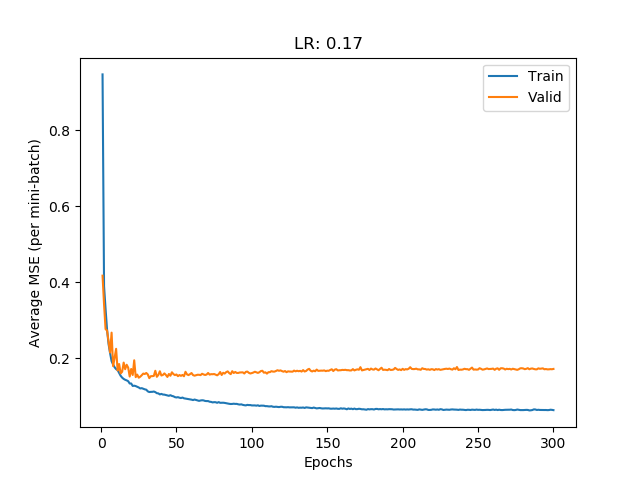
\includegraphics[width=0.5\textwidth]{figures/module4/testvtraining.png}
\caption{Comparison of accuracy on training and test sets for a neural network.}
\end{figure}

\section{Validation Details}
Terminology
\bi
\item \textbf{Training set:} the data that is used to fit each model. 
\item \textbf{Test set:} data not used in model fitting that is used to compare model accuracy. 
\item \textbf{Validation set (optional):} If you perform too many comparisons with the test set, you run the risk of overfitting the test data. A validation set is a third set of data that is also withheld and only used to validate the best one or two models based on the test set. 
\ei

Example in SAS: proc surveyselect allows cross validation to be used as a criteria for variable selection. 

\section{Cross Validation}
Whenever you have enough data, withholding a subset of the data prior to model building is ideal. 

\nspace
However, collecting new data can be very expensive such that creating a ``test set'' is not feasible. 

\textbf{Cross Validation:} is a method that tries to estimate test set error using training data. 

\nspace The process:
\bi 
\item Randomly separate our data into k-groups (usually five or ten). 
\item Treat all but one of the groups as a training set, the remaining group as a test set. 
\item Fit a model using the training data, predict for the test data. 
\item Repeat the process, each time treating a different group as the test data until all observations have a prediction. 
\ei

\nspace
SAS does not have an easy method for performing cross validation. For this purpose, we will stick to validation accuracy from a test set in our projects. 

\nspace
However, we have already used cross validation as a means of performing variable selection in proc glmselect. 

\nspace
\textbf{Cautions and Considerations:}
\bi
\item \textit{Any} variable selection techniques or other forms of training must be included as part of the cross validation process. In other words, you can't use all of the data to select variables, then act ``blind'' to that same data in the model validation step. 
\bi
\item The consequence of such a move is that you will likely overestimate your model's predictive capability. 
\item Trying to embed variable selection into cross validation is extraordinarily difficult and not necessarily stable. 
\item Check out this optional video for a more detailed explanation: \url{https://www.youtube.com/watch?v=r64tRyHFAJ8&list=PLOg0ngHtcqbPTlZzRHA2ocQZqB1D_qZ5V&index=23}
\ei
\item The more groups you create, the more models you must fit, which can get computationally expensive. 
\item Too many groups makes it hard to estimate the true ``test set'' error. 
\bi
\item Less groups, more bias, less variance in the test set error estimation. Try to select a number of cross validation groups that balance the bias and variance (usually five or ten groups). 
\ei
\item Check out chapter 5 in this book for more details on cross validation and other forms of model validation: 
\url{http://faculty.marshall.usc.edu/gareth-james/ISL/ISLR\%20Seventh\%20Printing.pdf}
\ei













% End the Document
%==============================================================================
\end{document}